% !TeX program = xelatex
% !TeX encoding = UTF-8
% ...existing code...
\documentclass[a4paper]{article}

\usepackage[UTF8]{ctex}
\usepackage[a4paper,margin=1in]{geometry}
\usepackage{graphicx}
\usepackage{float}
\usepackage{listings}
% \usepackage{listings-rust}
\usepackage{longtable}
\usepackage{booktabs}
\usepackage{hyperref}
\usepackage{fancyhdr}
\usepackage{lastpage}
\usepackage{color}
\usepackage{indentfirst}        % 首段缩进
\setlength{\parindent}{2em}     % 缩进2字符
\usepackage{zhnumber}           % 中文编号
\usepackage[dvipsnames,table,xcdraw]{xcolor}
\usepackage{adjustbox}
\usepackage{subcaption}
\usepackage{amsmath}
\usepackage{amssymb}
\usepackage[many]{tcolorbox}
% \newfontfamily{\enfont}{Arial}  % 定义英文字体
\usepackage{enumitem}
\usepackage{xeCJK}
\usepackage[T1]{fontenc}
\usepackage{lmodern}
\usepackage{inconsolata} % 使用更美观的等宽字体 Inconsolata
\usepackage{multirow} % 用于表格中的多行合并
\usepackage{tikz} % 添加 TikZ 宏包用于绘制流程图
\usetikzlibrary{positioning} % 添加定位库以支持 'of' 语法
\usepackage{array} % 提供 >{...} 列类型支持（修复表格中 \arraybackslash 的用法）

% 全局设置（影响所有级别）
\setlist[itemize]{
    itemsep=2pt,
    topsep=4pt,
    parsep=1pt,
    leftmargin=3em
}

% 仅设置第一级（最高级）
\setlist[itemize,1]{
    label=\textcolor{orange}{$\blacktriangleright$},
    font=\color{blue!80!black}\small\bfseries,
    before={\color{blue!80!black}\small\bfseries}
}

% 重置第二级及更深级别（恢复默认样式）
\setlist[itemize,2]{
    label={\normalfont\textbullet},
    font=\normalfont\normalsize\color{black},
    before={\color{black}},
    leftmargin=*
}
\setlist[itemize,3]{
    label={\normalfont$\circ$},
    font=\normalfont\normalsize,
    before={},
    leftmargin=*
}


% 定义可分页的引用环境
\newtcolorbox[auto counter]{myquote}[1][]{
    % breakable,                     % 允许跨页分断
    % enhanced jigsaw,               % 优化分页处的边框
    colback=gray!5,                % 背景色
    colframe=gray!30,              % 边框色
    left=5mm, right=5mm,           % 左右内边距
    top=3mm, bottom=3mm,           % 上下内边距
    width=0.85\textwidth,         % 宽度
    center,                     % 居中
    arc=0mm,                       % 直角边框
    boxrule=0.5pt,                 % 边框线宽
    fontupper=\small\linespread{1.1}\selectfont, % 行距微调（1.1倍）
    % fontupper=\sffamily\linespread{1.05}\selectfont, % 无衬线 + 紧凑行距
    before upper={\parindent2em\color{black!40!blue}\itshape\small\kaishu}, % 深蓝色文本
    #1 % 允许额外参数
}

%\newcommand{\college}{中山大学计算机学院}
\newcommand{\projname}{计算机网络实验|实验二}
\newcommand{\reporttitle}{静态路由}
\newcommand{\groupno}{第一组}
\newcommand{\authorname}{欧阳易芃、马福泉、刘昊、彭怡萱}
\newcommand{\major}{计算机科学与技术}
\newcommand{\adviser}{谢逸}
\newcommand{\startdate}{2025年10月20日}
\newcommand{\labenddate}{2025年10月25日}
\newcommand{\labroom}{实验D402}

\pagestyle{fancy} % 使用 fancyhdr 风格
\fancyhf{}      % 清空默认的页眉页脚

% 设置页眉
\fancyhead[L]{\kaishu \projname}      % 左侧页眉显示项目名称
\fancyhead[C]{\kaishu \reporttitle}    % 中间页眉显示报告标题
\fancyhead[R]{\kaishu \authorname} % 右侧页眉显示作者姓名

% 设置页脚
\fancyfoot[C]{第 \thepage 页，共 \pageref{LastPage} 页} % 中间页脚显示页码

% 去除页眉页脚与正文之间的分隔线
\renewcommand{\headrulewidth}{0.4pt}
\renewcommand{\footrulewidth}{0pt}

% 设置文档背景颜色
\definecolor{mybgcolor}{RGB}{0, 0, 0} % 定义背景颜色
\definecolor{NavyBlue}{RGB}{0,0,128} % 添加颜色定义



% 全局设置lstlisting的样式
\lstset{
    language=C, % 设置默认语言
    basicstyle=\footnotesize\ttfamily, % 设置字体族
    breaklines=true, % 自动换行
    keywordstyle=\bfseries\color{blue}, % 设置关键字为粗体，颜色为蓝色
    morekeywords={}, % 设置更多的关键字，用逗号分隔
    emph={}, % 指定强调词，如果有多个，用逗号隔开
    emphstyle=\bfseries\color{Rhodamine},
    commentstyle=\itshape\color{green!50!black},
    stringstyle=\bfseries\color{PineGreen!90!black},
    columns=fullflexible,% 设置列宽
    numbers=left,
    numbersep=2em,
    numberstyle=\footnotesize\color{gray},
    frame=single,
    framesep=1em,
    showstringspaces=false,% % 不显示字符串中的空格
    keepspaces=true,
    backgroundcolor=\color{gray!5},
    % linewidth=0.8\linewidth, % 设置宽度为当前行宽的 80%
    xleftmargin=0.2\linewidth, % 左右边距自动调整
    xrightmargin=0.08\linewidth,
    % gobble=2, % 可选：移除代码前的缩进
    % postbreak=\mbox{\textcolor{red}{$\hookrightarrow$}\space}, % 可选：换行符样式
    captionpos=b, % 可选：标题位置
    aboveskip=1em, % 可选：上方间距
    belowskip=1em, % 可选：下方间距
}

\begin{document}


% 封面
\begin{titlepage}
    \centering
    
    
\includegraphics[width=10cm]{img/SYSULogo.png}

    \vspace{1em}
    %{\Large \college \par}
    \vspace{1em}
    {\Large \kaishu \projname \par}
    \vspace{3em}

    {\fontsize{40pt}{42pt}\kaishu \selectfont \boldmath \reporttitle\par}
    \vspace*{\fill}

    \begin{center}
    {\Large
    \makebox[5em][s]{小组编号}:\underline{\makebox[15em][c]{\kaishu \groupno}}\\[1em]
    \makebox[5em][s]{组员姓名}:\underline{\makebox[15em][c]{\kaishu 欧阳易芃、马福泉}}\\[0.5em]
    \makebox[5em][s]{} \underline{\makebox[15em][c]{\kaishu 刘昊、彭怡萱}}\\[1em]
    \makebox[5em][s]{专业}:\underline{\makebox[15em][c]{\kaishu \major}}\\[1em]
    \makebox[5em][s]{课程教师}:\underline{\makebox[15em][c]{\kaishu \adviser}}\\[1em]
    \makebox[5em][s]{起始日期}:\underline{\makebox[15em][c]{\kaishu \startdate}}\\[1em]
    \makebox[5em][s]{结束日期}:\underline{\makebox[15em][c]{\kaishu \labenddate}}\\[1em]
    \makebox[5em][s]{实验地点}:\underline{\makebox[15em][c]{\kaishu \labroom}}
    }
    \end{center}

    \vspace*{\fill}
\end{titlepage}

% 目录
\tableofcontents
\newpage

\section{实验概述}

\subsection{实验目标}
\begin{itemize}
    \item 掌握通过静态路由方式实现网络的连通性。
    \item 掌握路由器静态路由的配置方法。
    \item 理解静态路由的工作原理。
\end{itemize}

\subsection{实验内容}
\begin{itemize}
    \item 完成本实验及实验思考。
    \item 在路由器 R1 和 R2 上配置静态路由，使 PC1 和 PC2 在跨路由器的情况下能互连互通。
    \item 配置之前，应该测试 2 台计算机的连通性，以便与配置后的连通性作对比。
\end{itemize}



根据实验要求，我们需要将两台主机通过路由器连接起来，形成一个简单的局域网。具体连接示意图如下所示：
\begin{figure}[H]
    \centering
    \adjustbox{
        max width=0.8\linewidth,
        max height=0.6\textheight,
        min width=1cm,
        min height=1cm,
        keepaspectratio
    }{
        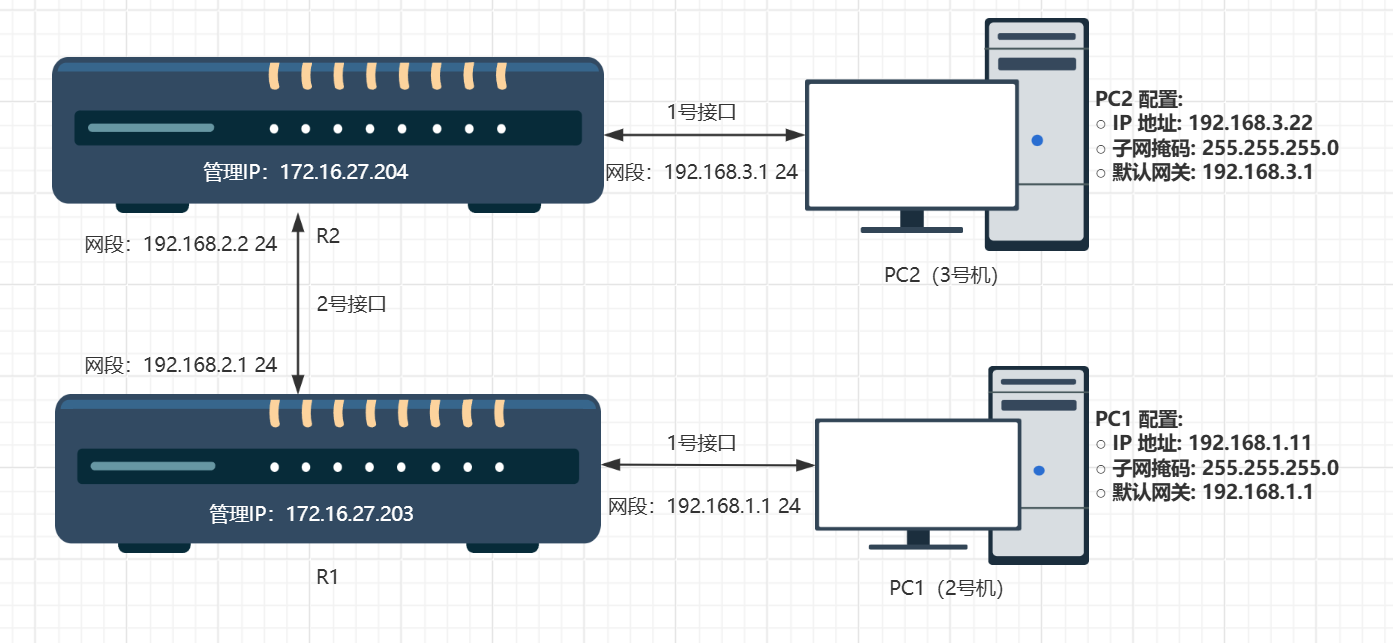
\includegraphics{img/figure_2.png}
    }
    \caption{主机与路由器连接示意图}
\end{figure}

\begin{itemize}
    \item PC1配置: 
    \begin{itemize}
        \item IP地址:192.168.1.11
        \item 子网掩码:255.255.255.0
        \item 默认网关:192.168.1.1
    \end{itemize}
    \item PC2配置:
    \begin{itemize}
        \item IP地址:192.168.3.22
        \item 子网掩码:255.255.255.0
        \item 默认网关:192.168.3.1
    \end{itemize}
    \item 路由器R1配置:
    \begin{itemize}
        \item 1号接口(连接PC1)地址：192.168.1.1/24
        \item 2号接口(连接R2)地址：192.168.2.1/24
    \end{itemize}
    \item 路由器R2配置:
    \begin{itemize}
        \item 1号接口(连接PC2)地址：192.168.3.1/24
        \item 2号接口(连接R1)地址：192.168.2.2/24
    \end{itemize}
\end{itemize}


\subsection{实验思考}
\begin{itemize}
    \item 在配置静态路由前，PC1 ping PC2，分析此时为何不通？
    \item 要实现 PC1和 PC2的通信，本实验共配置了几条静态路由？分别是什么？其含义是什么？
    \item 如果路由器中存在去往同一网段的多条路由信息，路由器会采用哪一个进行转发？
\end{itemize}

\section{静态路由原理详解}
\subsection{静态路由的基本概念}
静态路由是网络中最基础的路由方式之一，其核心是通过人工手动配置路由条目，指导路由器完成数据包的转发\cite{ref1}。与动态路由不同，静态路由不依赖于路由协议进行路由信息的交换和更新，而是由网络管理员根据网络拓扑结构和需求，手动设置每一条路由规则。这种方式虽然配置复杂且维护成本较高，但在小型网络或特定场景下，静态路由能够提供更高的安全性和可控性。

\subsection{静态路由的核心构成要素}
一个完整的静态路由条目需包含 3 个关键信息，共同决定数据包的转发路径：
\begin{table}[htbp]
\centering

\label{tab:static_route}
\begin{tabular}{|>{\raggedright\arraybackslash}p{0.25\textwidth}|>{\raggedright\arraybackslash}p{0.65\textwidth}|}
\hline
\textbf{构成要素} & \textbf{作用} \\
\hline
目标网络地址 / 子网掩码 & 定义需要到达的网络范围。例如 "192.168.2.1 255.255.255.1" 表示目标是 192.168.2.1网段。\\
\hline
出接口 & 数据包从本路由器的哪个物理/逻辑接口发送出去（如 GigabitEthernet 0/0/1）。\\
\hline
下一跳 IP 地址 & 数据包需要转发到的"下一个路由器接口的 IP 地址"（与出接口直接相连）。\\
\hline
\end{tabular}
\caption{静态路由构成要素及其作用}
\end{table}

\subsection{静态路由的工作流程}
\begin{figure}[H]
    \centering
    \adjustbox{
        max width=0.8\linewidth,
        max height=0.6\textheight,
        min width=1cm,
        min height=1cm,
        keepaspectratio
    }{
        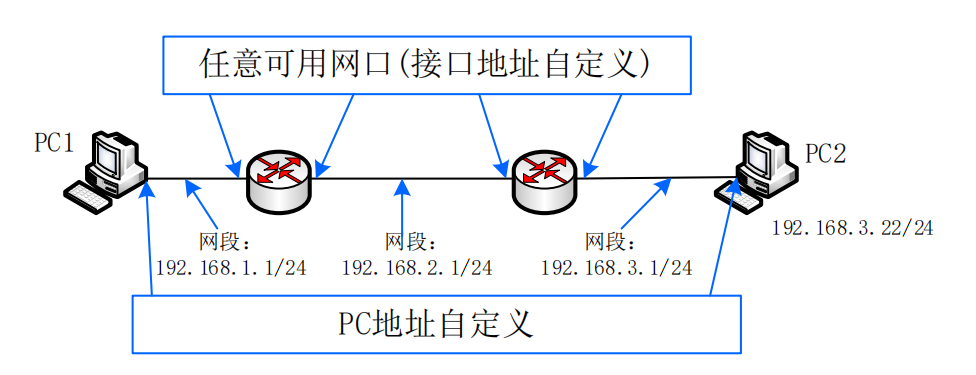
\includegraphics{img/figure_1.png}
    }
    \caption{静态路由拓扑图}
\end{figure}
\noindent \textbf{转发步骤:}
\begin{enumerate}
    \item 当 PC1 发送数据包到 PC2 时，数据包首先到达路由器 R1。
    \item \textbf{【关键步骤】路由表查找}：R1 检查其路由表，发现没有直接连接到 PC2 的路由条目。此步骤是整个转发过程的核心，路由器必须在路由表中找到匹配的条目才能继续转发。
    \item \textbf{【关键步骤】静态路由匹配}：R1 查找静态路由条目，找到去往 PC2 所在网段（192.168.3.0/24）的静态路由，确定下一跳为 R2 的 G0/2 接口（192.168.2.2）。这里体现了静态路由配置的重要性 - 如果没有正确配置这条路由，数据包将被丢弃。
    \item R1 将数据包通过 G0/2 接口发送到 R2。
    \item R2 接收到数据包后，检查其路由表，同样发现没有直接连接到 PC2 的路由条目。
    \item \textbf{【关键步骤】直连网络识别}：R2 查找路由表，发现 PC2 所在网段（192.168.3.0/24）是其直连网络，可以直接通过 G0/1 接口到达。这说明直连路由的优先级最高，无需额外配置。
    \item R2 将数据包通过 G0/1 接口发送到 PC2。
    \item PC2 接收到数据包，完成通信。
\end{enumerate}

\noindent \textbf{关键转发要点分析}：
\begin{itemize}
    \item \textbf{步骤2-3的重要性}：这两步决定了数据包能否成功转发。路由表查找失败或静态路由配置错误都会导致通信中断。
    \item \textbf{步骤6的特殊性}：当目标网络为直连网络时，路由器可以直接转发，无需查找静态路由，这体现了直连路由的最高优先级。
    \item \textbf{双向转发原理}：PC2回复PC1时，需要在R2上有对应的静态路由指向192.168.1.0/24网段，否则只能实现单向通信。
\end{itemize}

\section{实验步骤与结果}

\subsection{【步骤一】连接实验设备}
根据图2，我们需要将两台主机通过路由器连接起来，接口如下：
\begin{itemize}
    \item 主机2的网线连接到路由器R1的端口1
    \item 主机3的网线连接到路由器R2的端口1
    \item 路由器R1的端口2通过网线连接到路由器R2的端口2
\end{itemize}

\noindent\textbf{注意}：路由器的端口并不是顺序排列的，需要根据路由器上的标签进行连接，并且确保连接后的端口成功亮灯。

\subsection{【步骤二】为 PC 配置 IP 地址和掩码}
根据实验配置，我们手动配置两台主机的IP地址和子网掩码如下：

\begin{figure}[H]
    \centering
    % 第一张图片
    \begin{minipage}[t]{0.48\textwidth}
        \centering
        \adjustbox{
            max width=1.05\linewidth,
            max height=0.45\textheight,
            min width=1cm,
            min height=1cm,
            keepaspectratio
        }{
            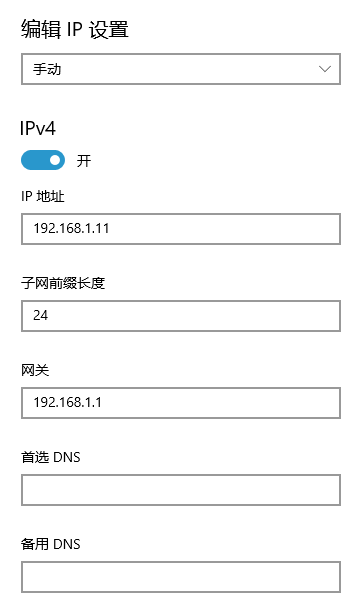
\includegraphics{img/PC1.png}
        }
        \subcaption{PC1配置}
    \end{minipage}
    \hfill
    % 第二张图片
    \begin{minipage}[t]{0.48\textwidth}
        \centering
        \adjustbox{
            max width=1\linewidth,
            max height=0.45\textheight,
            min width=1cm,
            min height=1cm,
            keepaspectratio
        }{
            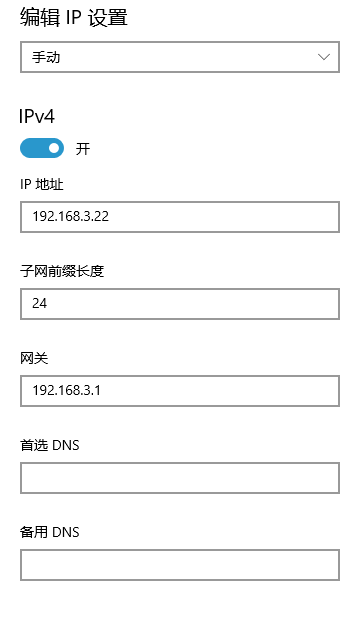
\includegraphics{img/PC2.png}
        }
        \subcaption{PC2配置}
    \end{minipage}
    \caption{主机配置}
\end{figure}

打开两台电脑并分别尝试ping对方的ip地址，发现不能ping通，因为路由器还未配置，路由表缺失，R1、R2找不到对方的路由，就会丢弃数据包。截图如下：

\begin{figure}[H]
    \centering
    % 第一张图片
    \begin{minipage}[t]{0.48\textwidth}
        \centering
        \adjustbox{
            max width=1.05\linewidth,
            max height=0.45\textheight,
            min width=1cm,
            min height=1cm,
            keepaspectratio
        }{
            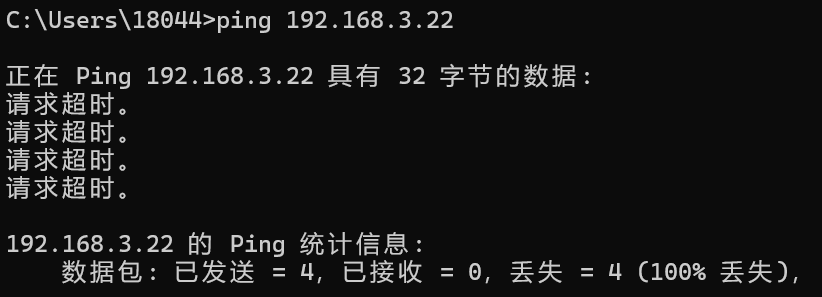
\includegraphics{img/ping2_3.png}
        }
        \subcaption{2号机ping3号机}
    \end{minipage}
    \hfill
    % 第二张图片
    \begin{minipage}[t]{0.48\textwidth}
        \centering
        \adjustbox{
            max width=1\linewidth,
            max height=0.45\textheight,
            min width=1cm,
            min height=1cm,
            keepaspectratio
        }{
            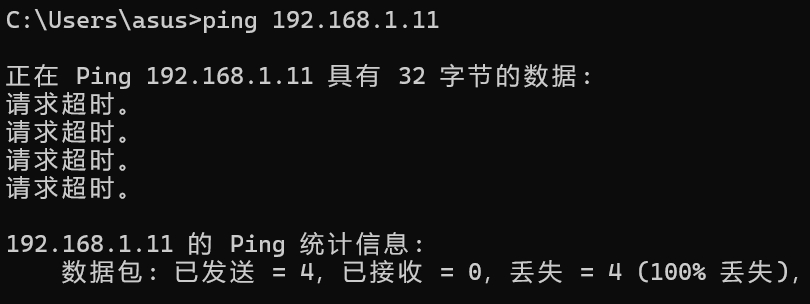
\includegraphics{img/ping3_2.png}
        }
        \subcaption{3号机ping2号机}
    \end{minipage}
    \caption{检查连接}
\end{figure}


\vspace{1em}
\subsection{【步骤三】配置路由器接口地址并开启接口}

根据实验要求，我们要分别在R1和R2上配置静态路由，使PC1和PC2能够互连互通。具体命令如下：

\begin{figure}[H]
  \centering
  \begin{minipage}[t]{0.48\textwidth}
    \begin{lstlisting}[language=C, xleftmargin=0pt]
Enter system view, return user view with Ctrl+Z.
//为R1配置静态路由
[AR6140-27-1]sysname R1

//进入接口1配置IP地址
[R2]interface GigabitEthernet0/0/1

[R2-GigabitEthernet0/0/1]ip address 192.168.1.1 24

[R2-GigabitEthernet0/0/1]undo shutdown

[R2-GigabitEthernet0/0/1]quit

//进入接口2配置IP地址
[R2]interface GigabitEthernet0/0/2

[R2-GigabitEthernet0/0/2]ip address 192.168.2.1 24

[R2-GigabitEthernet0/0/2]undo shutdown

[R2-GigabitEthernet0/0/2]quit
    \end{lstlisting}
    \subcaption{R1 配置}
  \end{minipage}\hfill
  \begin{minipage}[t]{0.48\textwidth}
    \begin{lstlisting}[language=C, xleftmargin=0pt]
Enter system view, return user view with Ctrl+Z.
//为R2配置静态路由
[AR6140-27-1]sysname R2

//进入接口1配置IP地址
[R2]interface GigabitEthernet0/0/1

[R2-GigabitEthernet0/0/1]ip address 192.168.3.1 24

[R2-GigabitEthernet0/0/1]undo shutdown

[R2-GigabitEthernet0/0/1]quit

//进入接口2配置IP地址
[R2]interface GigabitEthernet0/0/2

[R2-GigabitEthernet0/0/2]ip address 192.168.2.2 24

[R2-GigabitEthernet0/0/2]undo shutdown

[R2-GigabitEthernet0/0/2]quit
    \end{lstlisting}
    \subcaption{R2 配置}
  \end{minipage}
  \caption{R1 与 R2 接口配置}
\end{figure}

\noindent 配置结果如下：
\begin{figure}[H]
    \centering
    % 第一张图片
    \begin{minipage}[t]{0.48\textwidth}
        \centering
        \adjustbox{
            max width=1.05\linewidth,
            max height=0.45\textheight,
            min width=1cm,
            min height=1cm,
            keepaspectratio
        }{
            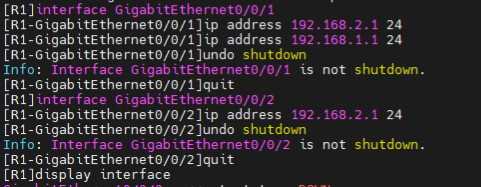
\includegraphics{img/order_1.png}
        }
        \subcaption{R1配置结果}
    \end{minipage}
    \hfill
    % 第二张图片
    \begin{minipage}[t]{0.48\textwidth}
        \centering
        \adjustbox{
            max width=1\linewidth,
            max height=0.45\textheight,
            min width=1cm,
            min height=1cm,
            keepaspectratio
        }{
            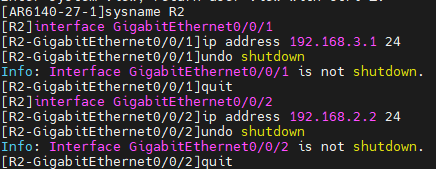
\includegraphics{img/order_2.png}
        }
        \subcaption{R2配置结果}
    \end{minipage}
    \caption{配置结果}
\end{figure}
接下来，我们通过\texttt{display interface}命令查看接口是否打开成功，若显示\texttt{UP}状态，则表示接口已成功打开。如下图所示：
\begin{figure}[H]
    \centering
    % 第一张图片
    \begin{minipage}[t]{0.48\textwidth}
        \centering
        \adjustbox{
            max width=1.05\linewidth,
            max height=0.45\textheight,
            min width=1cm,
            min height=1cm,
            keepaspectratio
        }{
            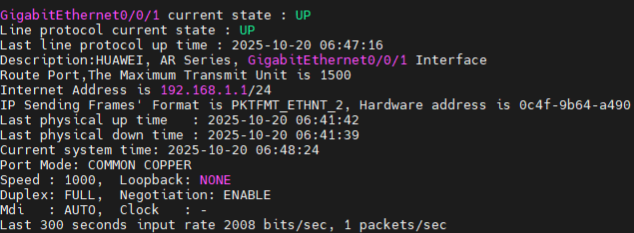
\includegraphics{img/result_1.1.png}
        }
        \subcaption{R1的1号接口}
    \end{minipage}
    \hfill
    % 第二张图片
    \begin{minipage}[t]{0.50\textwidth}
        \centering
        \adjustbox{
            max width=1\linewidth,
            max height=0.45\textheight,
            min width=1cm,
            min height=1cm,
            keepaspectratio
        }{
            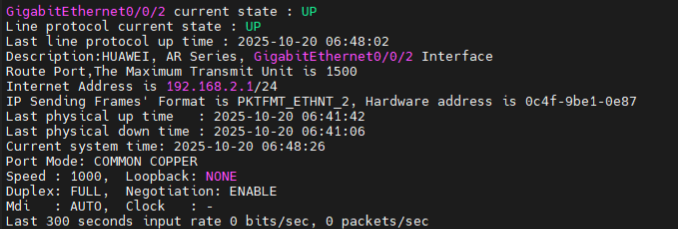
\includegraphics{img/result_1.2}
        }
        \subcaption{R1的2号接口}
    \end{minipage}
    \caption{R1接口状态检查}
\end{figure}

由图中可以看出，R1的两个接口均为UP状态，表示接口已成功打开。同理，我们也可以通过类似的命令检查R2的接口状态，确保其也处于UP状态。截图如下所示：
\begin{figure}[H]
    \centering
    % 第一张图片
    \begin{minipage}[t]{0.48\textwidth}
        \centering
        \adjustbox{
            max width=1.05\linewidth,
            max height=0.45\textheight,
            min width=1cm,
            min height=1cm,
            keepaspectratio
        }{
            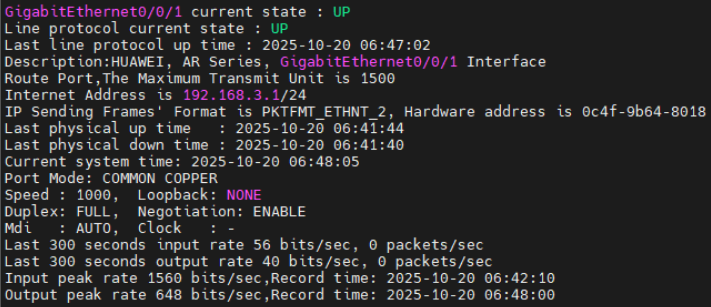
\includegraphics{img/result_2.1.png}
        }
        \subcaption{R2的1号接口}
    \end{minipage}
    \hfill
    % 第二张图片
    \begin{minipage}[t]{0.50\textwidth}
        \centering
        \adjustbox{
            max width=1\linewidth,
            max height=0.45\textheight,
            min width=1cm,
            min height=1cm,
            keepaspectratio
        }{
            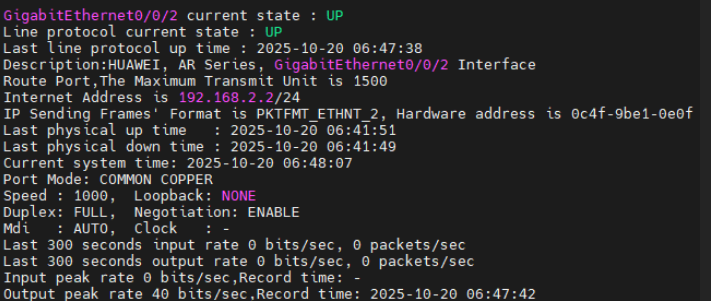
\includegraphics{img/result_2.2.png}
        }
        \subcaption{R2的2号接口}
    \end{minipage}
    \caption{R2接口状态检查}
\end{figure}

由图中可以看出，R2的两个接口均为UP状态，表示接口已成功打开。接下来，我们将继续配置静态路由，以实现PC1和PC2之间的通信。

\subsection{【步骤四】配置路由器静态路由}
\noindent 在 R1 上配置去往 PC2 所在网段的静态路由
\begin{itemize}
    \item 命令：[R1] ip route-static 192.168.3.0 24 192.168.2.2
\end{itemize}

\noindent 在 R2 上配置去往 PC1 所在网段的静态路由（回程路由）
\begin{itemize}
    \item 命令：[R2] ip route-static 192.168.1.0 24 192.168.2.1
\end{itemize}
\vspace{2em}
\noindent \textbf{静态路由的基本语法如下：}

ip route-static <目标网段IP地址> <子网掩码> <下一跳地址>

\noindent \textbf{解释：}

\begin{itemize}
    \item 对于[R1]而言：
    \begin{itemize}
        \item <目标网段IP地址>：192.168.3.22 \& 255.255.255.0 = 192.168.3.0
        \begin{itemize}
            \item 192.168.3.0 是网络地址,它本身不能分配给任何设备。
            \item 192.168.3.1 是第一个可用主机地址，在图中它被分配给了路由器R2的接口，作为这个网段的网关。
            \item 192.168.3.22 是另一个可用主机地址，分配给了PC2。
        \end{itemize}
        \item <子网掩码>：24 表示子网掩码为255.255.255.0 的一种简写形式，代表子网掩码在二进制形式下，从左边开始有 24个连续的 1。
        \item <下一跳地址>：192.168.2.2 （R2 的接口），表示数据包需要发送到的下一个路由器接口的 IP 地址。
    \end{itemize}
\end{itemize}   

\begin{itemize}
    \item 对于[R2]而言：
    \begin{itemize}
        \item <目标网段IP地址>：192.168.1.11 \& 255.255.255.0 = 192.168.1.0
        \begin{itemize}
            \item 192.168.1.0 是网络地址,它本身不能分配给任何设备。
            \item 192.168.1.1 是第一个可用主机地址，在图中它被分配给了路由器R1的接口，作为这个网段的网关。
            \item 192.168.1.11 是另一个可用主机地址，分配给了PC1。
        \end{itemize}
        \item <子网掩码>：24 表示子网掩码为255.255.255.0 的一种简写形式，代表子网掩码在二进制形式下，从左边开始有 24个连续的 1。
        \item <下一跳地址>：192.168.2.1 （R1 的接口），表示数据包需要发送到的下一个路由器接口的 IP 地址。
    \end{itemize}
\end{itemize}   

\vspace{1em}

\subsection{【步骤五】验证测试}
\subsubsection{查看路由表}
配置完成后，我们可以通过以下命令查看路由器的路由表，确认静态路由是否配置成功：
\begin{itemize}
    \item 命令：[R1] display ip routing-table
    \item 命令：[R2] display ip routing-table
\end{itemize}
得到的路由表截图如下所示：
\begin{figure}[H]
    \centering
    % 第一张图片
    \begin{minipage}[t]{0.48\textwidth}
        \centering
        \adjustbox{
            max width=1.05\linewidth,
            max height=0.45\textheight,
            min width=1cm,
            min height=1cm,
            keepaspectratio
        }{
            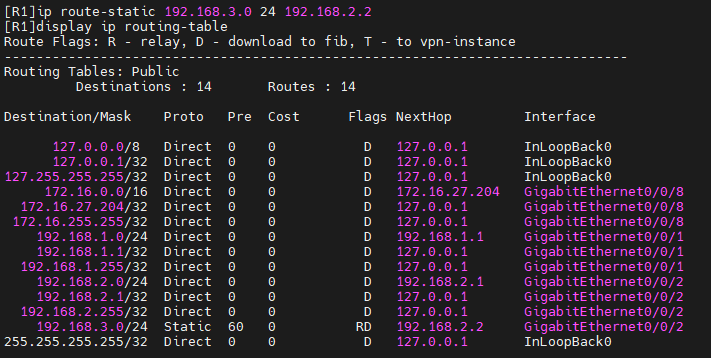
\includegraphics{img/route_table_1.png}
        }
        \subcaption{R1 路由表}
    \end{minipage}
    \hfill
    % 第二张图片
    \begin{minipage}[t]{0.48\textwidth}
        \centering
        \adjustbox{
            max width=1\linewidth,
            max height=0.45\textheight,
            min width=1cm,
            min height=1cm,
            keepaspectratio
        }{
            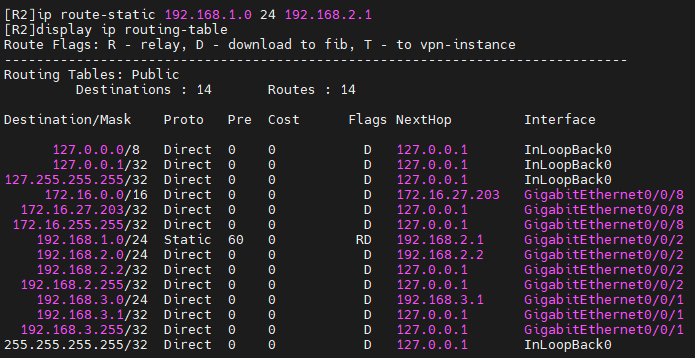
\includegraphics{img/route_table_2.png}
        }
        \subcaption{R2 路由表}
    \end{minipage}
    \caption{路由表检查}
\end{figure}    
由图中路由表输出可以确认静态路由已被正确添加，且路由器能够将去往对端网段的流量转发到相应的下一跳。为了便于阅读，这里对路由表中的关键字段作简要说明：
\begin{itemize}
    \item \textbf{Destination/Mask}：目标网络及其掩码（例如 192.168.3.0/24）。
    \item \textbf{Proto}：路由来源（Direct=直连，Static=静态等）。
    \item \textbf{Pre/Cost}：优先级/代价值，用于路由选择（数值越小优先级越高或代价越低，具体含义因厂商略有不同）。
    \item \textbf{Flags}：路由标志，表明该路由的状态或属性（例如 D 表示直连，R 表示可路由等）。
    \item \textbf{NextHop}：下一跳地址（数据包应发送到的下一个设备 IP）。
    \item \textbf{Interface}：出接口（路由器用于转发该条目的物理/逻辑端口）。
\end{itemize}

下面给出实验指导中 R1 的关键输出部分：
\begin{verbatim}
Destination/Mask   Proto   Pre Cost Flags NextHop        Interface
192.168.1.0/24     Direct  0   0    D     192.168.1.1   Ethernet0/0/1
192.168.2.0/24     Direct  0   0    D     192.168.2.1   Ethernet0/0/2
192.168.3.0/24     Static  60  0    RD    192.168.2.2   Ethernet0/0/2
\end{verbatim}

其中前两条（192.168.1.0/24 与 192.168.2.0/24）为本路由器的直连网络，由接口配置自动产生；第三条（192.168.3.0/24）为本次实验手动添加的静态路由，下一跳为 192.168.2.2（即 R2 在互联网段上的接口）。R2 上也应有对应的回程静态路由（将 192.168.1.0/24 指向 192.168.2.1）。

当这些条目存在且下一跳可达时，R1 与 R2 就能完成逐跳转发，PC1 与 PC2 之间的 ICMP 测试（ping）也将成功，从而证明静态路由配置正确有效。
\subsubsection{测试端到端连通性}
配置完成后，我们再次尝试从 PC1 ping PC2，验证两台主机之间的连通性。截图如下所示：
\begin{figure}[H]
    \centering
    \adjustbox{
        max width=0.8\linewidth,
        max height=0.6\textheight,
        min width=1cm,
        min height=1cm,
        keepaspectratio
    }{
        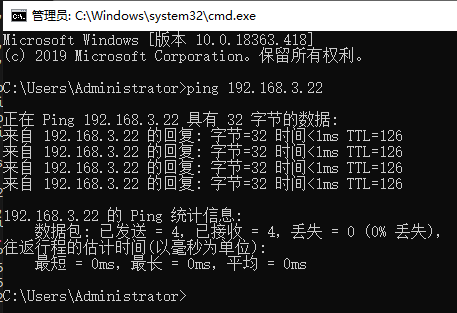
\includegraphics{img/image.png}
    }
    \caption{PC1 ping PC2 结果}
\end{figure}

由图中可以看出，PC1 和 PC2 之间的 ping 测试均成功，表示两台主机之间已经实现了互连互通，静态路由配置正确有效。

本次实验，我们搭建了一个简单的静态路由网络，逐步完成了以下关键步骤：

\begin{enumerate}
    \item 首先，我们根据实验拓扑图连接了实验设备，确保了物理连接的正确性。接着，为两台主机手动配置了 IP 地址和子网掩码，并验证了初始状态下主机之间无法通信的现象。这一步帮助我们理解了路由器在网络通信中的重要作用。

    \item 随后，我们为路由器的各个接口配置了 IP 地址，并开启了接口，使得路由器能够正常工作。通过检查接口状态，我们确认了接口的配置无误。

    \item 接下来，我们在两台路由器上分别配置了静态路由。R1 上的静态路由指向 PC2 所在的网段，而 R2 上的静态路由则指向 PC1 所在的网段。这些静态路由的配置使得路由器能够根据目标地址正确地转发数据包。

    \item 最后，我们通过查看路由表验证了静态路由的配置结果，并进行了端到端的连通性测试。测试结果表明，PC1 和 PC2 之间的通信已经成功实现。
 
\end{enumerate}
\section{实验思考}
\begin{enumerate}
    \item 在配置静态路由前，PC1 ping PC2，分析此时为何不通？

    \begin{myquote}[colback=blue!5!white,colframe=blue!75!black,title=回答]
    \textbf{核心原因}：路由信息缺失导致数据包无法正确转发。
    
    \textbf{详细分析}：
    \begin{itemize}
        \item \textbf{路由表状态}：初始状态下，R1和R2的路由表中只包含直连网络的路由信息，缺少跨路由器网段的路由条目
        \item \textbf{数据包传输过程}：当PC1（192.168.1.11）向PC2（192.168.3.22）发送数据包时，R1接收到数据包后查找路由表，发现没有到达192.168.3.0/24网段的路由信息
        \item \textbf{转发决策失败}：R1无法确定将数据包发送到哪个下一跳，根据路由协议的默认行为，将该数据包丢弃
        \item \textbf{通信中断}：由于数据包在R1处被丢弃，PC2永远收不到来自PC1的数据包，因此ping测试失败
    \end{itemize}
    
    \textbf{本质原因}：这体现了路由器作为三层设备的核心功能 - 只有当路由表中存在到达目标网络的路由条目时，路由器才能完成数据包的转发。
    \end{myquote}

    \item 要实现 PC1 和 PC2 的通信，本实验共配置了几条静态路由？分别是什么？其含义是什么？

    \begin{myquote}[colback=green!5!white,colframe=green!75!black,title=回答]
    \textbf{配置数量}：本实验共配置了2条静态路由。
    
    \textbf{具体配置及含义}：
    \begin{enumerate}
        \item \textbf{R1上的静态路由}：
        \begin{itemize}
            \item 配置命令：\texttt{ip route-static 192.168.3.0 24 192.168.2.2}
            \item 路由含义：告诉R1，当需要访问192.168.3.0/24网段时，将数据包发送给下一跳路由器192.168.2.2（即R2在中间网段的接口）
            \item 作用：实现从PC1到PC2方向的数据包转发
        \end{itemize}
        
        \item \textbf{R2上的静态路由}：
        \begin{itemize}
            \item 配置命令：\texttt{ip route-static 192.168.1.0 24 192.168.2.1}
            \item 路由含义：告诉R2，当需要访问192.168.1.0/24网段时，将数据包发送给下一跳路由器192.168.2.1（即R1在中间网段的接口）
            \item 作用：实现从PC2到PC1方向的数据包转发（回程路由）
        \end{itemize}
    \end{enumerate}
    
    \textbf{双向通信原理}：
    \begin{itemize}
        \item 这两条路由相互配合，形成完整的双向通信路径
        \item 缺少任何一条路由都会导致单向通信失败
        \item 体现了网络通信中"有来有回"的基本原则
    \end{itemize}
    \end{myquote}

    \item 如果路由器中存在去往同一网段的多条路由信息，路由器会采用哪一个进行转发？

    \begin{myquote}[colback=yellow!5!white,colframe=yellow!75!black,title=回答]
    \textbf{路由选择遵循的优先级顺序}：
    
    \begin{enumerate}
        \item \textbf{最长前缀匹配原则（Longest Prefix Match）}：
        \begin{itemize}
            \item 优先选择子网掩码最长（最具体）的路由条目
            \item 例如：同时存在192.168.1.0/24和192.168.1.0/16两条路由时，选择/24的路由
            \item 原理：更长的前缀意味着更精确的匹配
        \end{itemize}
        
        \item \textbf{管理距离/优先级比较（Administrative Distance）}：
        \begin{itemize}
            \item 当前缀长度相同时，比较路由的管理距离（Pre字段）
            \item 数值越小，可信度越高，优先级越高
            \item 常见优先级：直连路由(0) > 静态路由(1) > 动态路由协议(>1)
        \end{itemize}
        
        \item \textbf{路由度量值比较（Metric/Cost）}：
        \begin{itemize}
            \item 当管理距离也相同时，比较路由的代价值
            \item 选择代价最小的路由进行转发
            \item 代价可能基于带宽、跳数、延迟等因素计算
        \end{itemize}
        
        \item \textbf{负载均衡或其他策略}：
        \begin{itemize}
            \item 若以上条件完全相同，路由器可能采用等价路径负载均衡（ECMP）
            \item 或根据厂商实现选择特定路由（如接口编号较小者）
        \end{itemize}
    \end{enumerate}
    
    \textbf{实际应用示例}：
    在华为设备中，可通过路由表的Pre/Cost字段观察路由优先级，直连路由的Pre为0，静态路由的Pre通常为60，这解释了为什么直连路由总是优先于静态路由被选择。
    \end{myquote}

\end{enumerate}

\section{实验总结}

通过本次静态路由实验，我们小组掌握了静态路由的基本配置方法，深入理解了路由器数据包转发的工作原理，并培养了网络故障排查和团队协作能力。

\subsection{实验过程中的注意事项与经验总结}

\subsubsection{物理连接与设备准备}
\begin{itemize}
    \item \textbf{端口识别与连接}：路由器端口编号可能不连续，必须仔细查看设备标签，确保连接到正确的物理端口。连接后观察端口指示灯状态，亮灯表示物理连接正常。
    \item \textbf{设备启动顺序}：建议先启动路由器，后启动PC，确保所有设备完全启动后再进行配置，避免因设备未就绪导致的配置失败。
    \item \textbf{线缆质量检查}：使用质量良好的网线，避免因线缆问题导致的间歇性连接故障。
\end{itemize}

\subsubsection{配置操作要点}
\begin{itemize}
    \item \textbf{命令语法准确性}：静态路由配置命令的参数顺序和格式必须严格准确，特别注意IP地址和子网掩码的正确写法（如24与255.255.255.0的对应关系）。
    \item \textbf{接口激活的重要性}：配置IP地址后必须使用\texttt{undo shutdown}命令激活接口，这是初学者最容易忽略的步骤。
    \item \textbf{双向路由配置}：必须在两台路由器上都配置相应的静态路由，确保数据包能够往返，缺少任何一条都会导致单向通信失败。
    \item \textbf{下一跳地址验证}：下一跳地址必须是与当前路由器直连网段内的有效IP地址，且该地址必须是可达的。
\end{itemize}

本次实验为我们后续学习奠定了坚实基础，掌握的故障排查方法和网络思维将在更复杂的网络环境中发挥重要作用。

% ...existing code...
\begin{thebibliography}{99}  
    \bibitem{ref1}CSDN博客. (2025). 静态路由的原理详解（包含实例解析）. \url{https://blog.csdn.net/t_suifeng/article/details/149194906}
    \bibitem{ref2}Yi Xie. (2025). 中山大学计算机网络实验课程.
    

\end{thebibliography}


\end{document}